\chapter{ArcFace}\label{ch:arcface}
ArcFace~\cite{ArcFace} is a research which became public in 2018 and achieved state-of-the-art results on LFW dataset.
The objective of the research was to design a loss function which solves the main drawbacks of \textit{sofmax loss}
and the \textit{triplet loss}.

There are two issues with \textit{softmax loss}.
The first one is that the dimension of the output weight matrix grows linearly with the number of identities in the
training set.
The second drawback is that the learned features are not discriminative enough for the open-set face recognition
problem.
That means that the model doesn't perform well on not yet seen faces.

The drawbacks of \textit{triplet loss} are the demands entailed by the construction of the triplets.
The number of those is subject to combinatorial explosion.
This is a serious issue especially for large datasets.

ArcLoss is based on the equation of \textit{softmax loss}~\ref{eq:softmax}.
There are few steps separating the original and the improved version:
\begin{enumerate}
    \item First step is to fix the bias $b_j = 0$.
    \item Then we transform the logit as $W_j^T x_i = \norm{W_j} \norm{x_j} cos \theta_j$
    $\theta$ is the angle between the weight $W_j$ and the feature $x_i$.
    \item In a third step we fix the individual weights $\norm{W_j} = 1$ by $l_2$ normalization
    \item We do the same for feature $x_i$ and re-scale it to $s$ where coefficient $s$ is predetermined feature scale.
    These normalization steps make the prediction depend only on the angle $\theta$.
    The embeddings are distributed on the hypersphere with a radius $s$.
\end{enumerate}

\begin{figure}[H]
    \centering
    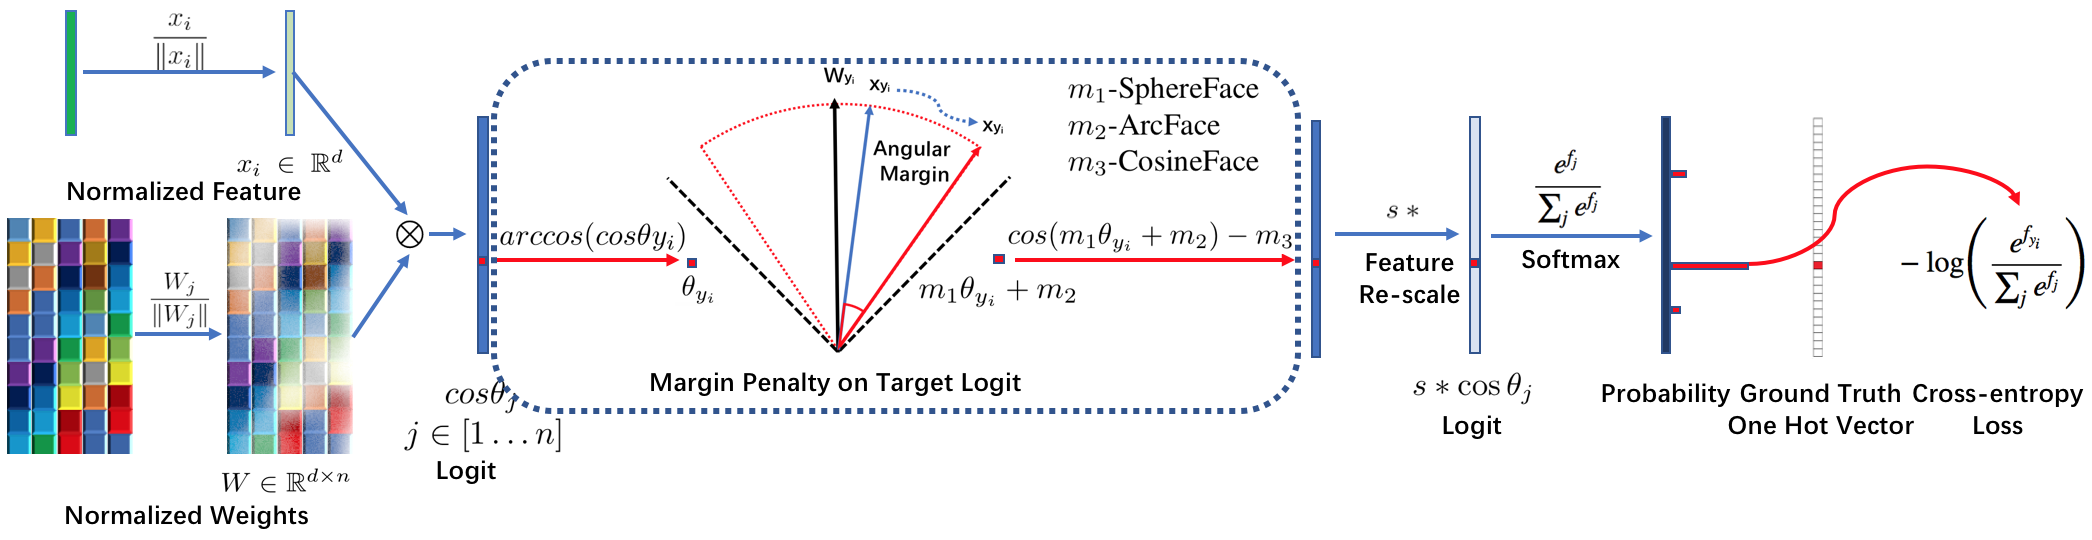
\includegraphics[width=\columnwidth]{images/arcface/arcface.png}
    \caption{Training a CNN for face recognition supervised by the ArcFace loss~\cite{ArcFace}}
    \label{fig:arcface}
\end{figure}